%\tikzset{every picture/.style={line width=0.75pt}} %set default line width to 0.75pt        

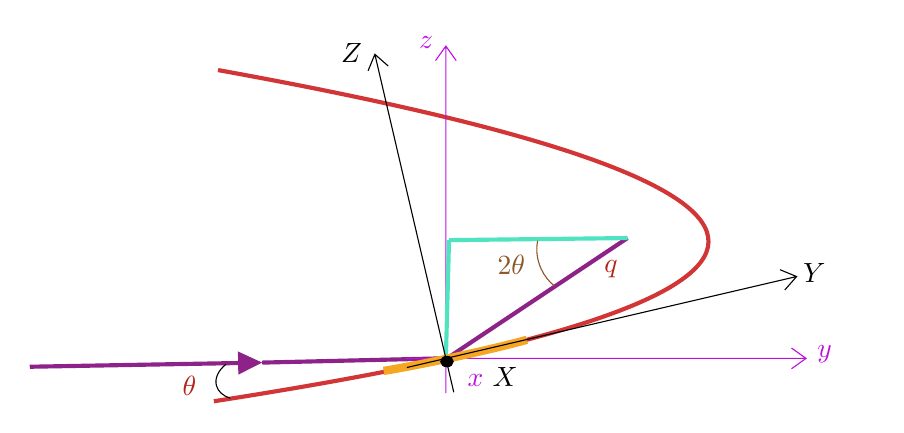
\begin{tikzpicture}[x=0.75pt,y=0.75pt,yscale=-1,xscale=1]
%uncomment if require: \path (0,214); %set diagram left start at 0, and has height of 214

%Shape: Parabola [id:dp636758281566334] 
\draw  [color={rgb, 255:red, 209; green, 53; blue, 53 }  ,draw opacity=1 ][line width=1.5]  (215.73,193.63) .. controls (532.78,144.36) and (533.44,91.17) .. (217.71,34.06) ;
%Straight Lines [id:da5751643928734858] 
\draw [color={rgb, 255:red, 141; green, 34; blue, 137 }  ,draw opacity=1 ][line width=1.5]    (239,175) -- (324,173) ;
%Straight Lines [id:da4985393188459284] 
\draw [color={rgb, 255:red, 141; green, 34; blue, 137 }  ,draw opacity=1 ][line width=1.5]    (328,173) -- (415,115) ;
%Shape: Axis 2D [id:dp5339485321600788] 
\draw [color={rgb, 255:red, 189; green, 16; blue, 224 }  ,draw opacity=1 ] (308.2,172.98) -- (501,172.98)(327.48,22.53) -- (327.48,189.7) (494,167.98) -- (501,172.98) -- (494,177.98) (322.48,29.53) -- (327.48,22.53) -- (332.48,29.53)  ;
%Straight Lines [id:da984423242776999] 
\draw [color={rgb, 255:red, 141; green, 34; blue, 137 }  ,draw opacity=1 ][line width=1.5]    (127,177) -- (235,175.07) ;
\draw [shift={(239,175)}, rotate = 538.98] [fill={rgb, 255:red, 141; green, 34; blue, 137 }  ,fill opacity=1 ][line width=0.08]  [draw opacity=0] (11.61,-5.58) -- (0,0) -- (11.61,5.58) -- cycle    ;
%Straight Lines [id:da25833218941129754] 
\draw [color={rgb, 255:red, 80; green, 227; blue, 194 }  ,draw opacity=1 ][line width=1.5]    (329,116) -- (415,115) ;
%Straight Lines [id:da4020633150416717] 
\draw [color={rgb, 255:red, 80; green, 227; blue, 194 }  ,draw opacity=1 ][line width=1.5]    (329,116) -- (327.48,172.98) ;
%Shape: Arc [id:dp507008334854385] 
\draw  [draw opacity=0] (379.83,138.12) .. controls (377.17,136.02) and (374.91,133.19) .. (373.35,129.77) .. controls (371.31,125.28) and (370.83,120.52) .. (371.71,116.28) -- (389.13,122.59) -- cycle ; \draw  [color={rgb, 255:red, 139; green, 87; blue, 42 }  ,draw opacity=1 ] (379.83,138.12) .. controls (377.17,136.02) and (374.91,133.19) .. (373.35,129.77) .. controls (371.31,125.28) and (370.83,120.52) .. (371.71,116.28) ;
%Shape: Arc [id:dp28668965321519213] 
\draw  [draw opacity=0] (223.6,192.18) .. controls (220.17,191.08) and (217.66,188.93) .. (216.92,186.03) .. controls (216.01,182.5) and (217.91,178.69) .. (221.55,175.8) -- (232.39,182.04) -- cycle ; \draw   (223.6,192.18) .. controls (220.17,191.08) and (217.66,188.93) .. (216.92,186.03) .. controls (216.01,182.5) and (217.91,178.69) .. (221.55,175.8) ;
%Curve Lines [id:da06756156046542072] 
\draw [color={rgb, 255:red, 245; green, 166; blue, 35 }  ,draw opacity=1 ][line width=3]    (297.5,179) .. controls (318.17,175.67) and (355.17,167.33) .. (366.5,164) ;
%Shape: Axis 2D [id:dp06708045637689208] 
\draw [color={rgb, 255:red, 0; green, 0; blue, 0 }  ,draw opacity=1 ] (308.7,177.37) -- (496.46,133.54)(293.28,26.46) -- (331.28,189.26) (488.5,130.26) -- (496.46,133.54) -- (490.78,140) (290,34.42) -- (293.28,26.46) -- (299.74,32.14)  ;
%Shape: Ellipse [id:dp8232202429248765] 
\draw  [fill={rgb, 255:red, 0; green, 0; blue, 0 }  ,fill opacity=1 ] (325,174.5) .. controls (325,173.12) and (326.34,172) .. (328,172) .. controls (329.66,172) and (331,173.12) .. (331,174.5) .. controls (331,175.88) and (329.66,177) .. (328,177) .. controls (326.34,177) and (325,175.88) .. (325,174.5) -- cycle ;

% Text Node
\draw (510,171) node  [color={rgb, 255:red, 179; green, 35; blue, 24 }  ,opacity=1 ,rotate=-359.63]  {$\textcolor[rgb]{0.74,0.06,0.88}{y}$};
% Text Node
\draw (318,21) node  [color={rgb, 255:red, 179; green, 35; blue, 24 }  ,opacity=1 ,rotate=-359.63]  {$\textcolor[rgb]{0.74,0.06,0.88}{z}$};
% Text Node
\draw (282,26) node  [color={rgb, 255:red, 179; green, 35; blue, 24 }  ,opacity=1 ,rotate=-359.63]  {$\textcolor[rgb]{0,0,0}{Z}$};
% Text Node
\draw (505,132) node  [color={rgb, 255:red, 179; green, 35; blue, 24 }  ,opacity=1 ,rotate=-359.63]  {$\textcolor[rgb]{0,0,0}{Y}$};
% Text Node
\draw (350,182) node  [color={rgb, 255:red, 179; green, 35; blue, 24 }  ,opacity=1 ,rotate=-359.63]  {$\textcolor[rgb]{0.74,0.06,0.88}{x} \ \textcolor[rgb]{0,0,0}{X}$};
% Text Node
\draw (407,130) node  [color={rgb, 255:red, 179; green, 35; blue, 24 }  ,opacity=1 ,rotate=-359.63]  {$q$};
% Text Node
\draw (204,186) node  [color={rgb, 255:red, 179; green, 35; blue, 24 }  ,opacity=1 ,rotate=-359.63]  {$\theta $};
% Text Node
\draw (359,128) node  [color={rgb, 255:red, 139; green, 87; blue, 42 }  ,opacity=1 ,rotate=-359.63]  {$2\theta $};


\end{tikzpicture}

